\documentclass[cs4size,a4paper]{ctexart}   
%==================== 数学符号公式 ============
\usepackage{amsmath}                 % AMS LaTeX宏包
\usepackage[style=1]{mdframed}
\usepackage{amsthm}
\usepackage{amsfonts}
\usepackage{mathrsfs}                % 英文花体字体
\usepackage{bm}                      % 数学公式中的黑斜体
\usepackage{bbding,manfnt}           % 一些图标,如 \dbend
\usepackage{lettrine}                % 首字下沉,命令\lettrine
\def\attention{\lettrine[lines=2,lraise=0,nindent=0em]{\large\textdbend\hspace{1mm}}{}}
\usepackage{longtable}
\usepackage[toc,page]{appendix}
\usepackage{geometry}                % 页边距调整
\usepackage{makecell}                % 表格内换行
\geometry{top=3.0cm,bottom=2.7cm,left=2.5cm,right=2.5cm}
%====================公式按章编号==========================
\numberwithin{equation}{section}
\numberwithin{table}{section}
\numberwithin{figure}{section}
%================= 基本格式预置 ===========================
\usepackage{fancyhdr}
\pagestyle{fancy}
\fancyhf{}  
\fancyhead[C]{\zihao{5}  \kaishu fancyhead千万别忘改了}
\fancyfoot[C]{~\zihao{5} \thepage~}
\renewcommand{\headrulewidth}{0.65pt} 
% \CTEXsetup[format={\centering\bfseries\zihao{-2}},name={第, 章}]{section}
\CTEXsetup[format={\centering\bfseries\zihao{4}}]{section}
\CTEXsetup[format={\bfseries \zihao{4}}]{subsection}
\CTEXsetup[format={\bfseries \zihao{-4}}]{subsubsection}
%================== 图形支持宏包 =========================
\usepackage{subfig}
\usepackage{graphicx}                % 嵌入png图像
\usepackage{color,xcolor}            % 支持彩色文本、底色、文本框等
\usepackage{hyperref}                % 交叉引用
\usepackage{caption}
\captionsetup{figurewithin=section}
%==================== 源码和流程图 =====================
\usepackage{listings}                % 粘贴源代码
\usepackage{xcolor}
\usepackage{color}
\definecolor{dkgreen}{rgb}{0,0.6,0}
\definecolor{gray}{rgb}{0.5,0.5,0.5}
\definecolor{mauve}{rgb}{0.58,0,0.82}
 \usepackage{xcolor}

% \renewcommand{\lstlistingname}{代码}    % 代码标题样式修改无效?!
%  \lstset{
%     basicstyle          =   \sffamily,          % 基本代码风格
%     keywordstyle        =   \bfseries,          % 关键字风格
%     commentstyle        =   \rmfamily\itshape,  % 注释的风格,斜体
%     stringstyle         =   \ttfamily,  % 字符串风格
%     flexiblecolumns,                % 别问为什么,加上这个
%     numbers             =   left,   % 行号的位置在左边
%     showspaces          =   false,  % 是否显示空格,显示了有点乱,所以不现实了
%     numberstyle         =   \zihao{5}\ttfamily,    % 行号的样式,小五号,tt等宽字体
%     showstringspaces    =   false,
%     captionpos          =   t,      % 这段代码的名字所呈现的位置,t指的是top上面
%     frame               =   lrtb,   % 显示边框
% }

%  \lstdefinestyle{SPICE}{
%     language        =   matlab, % 语言选Python
%     basicstyle      =   \zihao{-5}\ttfamily,
%     numberstyle     =   \zihao{-5}\ttfamily,
%     keywordstyle    =   \color{blue},
%     keywordstyle    =   [2] \color{teal},
%     stringstyle     =   \color{magenta},
%     commentstyle    =   \color{red}\ttfamily,
%     breaklines      =   true,   % 自动换行,建议不要写太长的行
%     columns         =   fixed,  % 如果不加这一句,字间距就不固定,很丑,必须加
%     basewidth       =   0.5em,
% }

%--------------------
\hypersetup{hidelinks}
\usepackage{booktabs}  
\usepackage{shorttoc}
\usepackage{tabu,tikz}
\usepackage{float}

\usepackage{multirow}



\tabcolsep=1ex
\tabulinesep=\tabcolsep
\newlength\tikzboxwidth
\newlength\tikzboxheight
\newcommand\tikzbox[1]{%
        \settowidth\tikzboxwidth{#1}%
        \settoheight\tikzboxheight{#1}%
        \begin{tikzpicture}
        \path[use as bounding box]
                (-0.5\tikzboxwidth,-0.5\tikzboxheight)rectangle
                (0.5\tikzboxwidth,0.5\tikzboxheight);
        \node[inner sep=\tabcolsep+0.5\arrayrulewidth,line width=0.5mm,draw=black]
                at(0,0){#1};
        \end{tikzpicture}%
        }

\makeatletter
\def\hlinew#1{%
  \noalign{\ifnum0=`}\fi\hrule \@height #1 \futurelet
   \reserved@a\@xhline}
   
\newcommand{\tabincell}[2]{\begin{tabular}{@{}#1@{}}#2\end{tabular}}%

\usepackage{subfig}

\usepackage{CJK}
\usepackage{ifthen}


\usepackage{graphicx} 
\newcommand{\HRule}{\rule{\linewidth}{0.5mm}}

\newtheorem{Theorem}{定理}
\newtheorem{Lemma}{引理} 
%%使得公式随章节自动编号
\makeatletter
\@addtoreset{equation}{section}
\makeatother
\renewcommand{\theequation}{\arabic{section}.\arabic{equation}}

%-------------------------
	
\usepackage{pythonhighlight}
\usepackage{tikz}                    
\usepackage{tikz-3dplot}
\usetikzlibrary{shapes,arrows,positioning}
%===================   正文开始    ===================
\begin{document}
\bibliographystyle{gbt7714-2005}     %论文引用格式
%===================  定理类环境定义 ===================
\newtheorem{example}{例}              % 整体编号
\newtheorem{algorithm}{算法}
\newtheorem{theorem}{定理}            % 按 section 编号
\newtheorem{definition}{定义}
\newtheorem{axiom}{公理}
\newtheorem{property}{性质}
\newtheorem{proposition}{命题}
\newtheorem{lemma}{引理}
\newtheorem{corollary}{推论}
\newtheorem{remark}{注解}
\newtheorem{condition}{条件}
\newtheorem{conclusion}{结论}
\newtheorem{assumption}{假设}
%==================重定义 ===================
\renewcommand{\contentsname}{目录}     
\renewcommand{\abstractname}{摘要} 
\renewcommand{\refname}{参考文献}     
\renewcommand{\indexname}{索引}
\renewcommand{\figurename}{图}
\renewcommand{\tablename}{表}
\renewcommand{\appendixname}{附录}
\renewcommand{\proofname}{证明}
\renewcommand{\algorithm}{算法} 
%============== 封皮和前言 =================
% \input{body/cover}
\pagestyle{plain}
\pagenumbering{arabic}
% \include{body/abstract}
\pagestyle{empty}
% \tableofcontents 
% \thispagestyle{empty}
%============== 论文正文   =================
% \pagestyle{fancy}
\pagestyle{plain}
% \include{body/chapter1}      %
% \include{body/chapter2}
% \include{body/chapter3}
% \include{body/chapter4}
% \include{body/chapter5}
% \include{body/chapter6}

\begin{center}
    \textsc{\zihao{-3} \bfseries ADDA课程项目}\\[0.3cm]
\end{center}

\begin{center}
	组员:冯俊杰、贾梓越、陈江华、陈畅
\end{center}

\section{设计目标}
\noindent
研究内容:

通过 matlab 建模或者 cadence(MOS 管级/verilogA 级,工艺不限)构建一个时钟交
织 Pipelined-SAR ADC,pipelined 级数不限,时钟校准通道数≥4 条,精度≥12 位,
TI-ADC 总采样率≥2GS/s,自己手动添加以下误差和失配,例如采样时钟 jitter 范围
100fs~5ps,timing skew 范围 200fs~5ps, inter-stage gain error± 10%等(以上参
数仅供参考), 通过静态分析方法和动态分析方法分析:TI mismatch (gain mismatch,
offset mismatch and timing skew), pipelined-SAR ADC 级间增益误差(inter-stage 
gain error), 第一级 SAR ADC 电容失配(capacitor-DAC mismatch),比较器失调,
时钟 jitter 等的影响。选择一种 time skew 校准方法进行 timing skew 误差检测并分
析。建模、仿真验证、撰写完整分析报告,在 cadence 里面完成仿真验证的有额外 bonus
分数。

\noindent
分析方法:

静态特性分析:转移特性曲线/统计方法;动态特性分析:FFT

\section{电路结构及原理}

    \subsection{Pipeline SAR ADC建模原理}
        基本架构:如图\ref{fig:circuit1}所示,两级SAR级间插入一个余量放大器。
        	\begin{figure}[H]
        		\centering
        		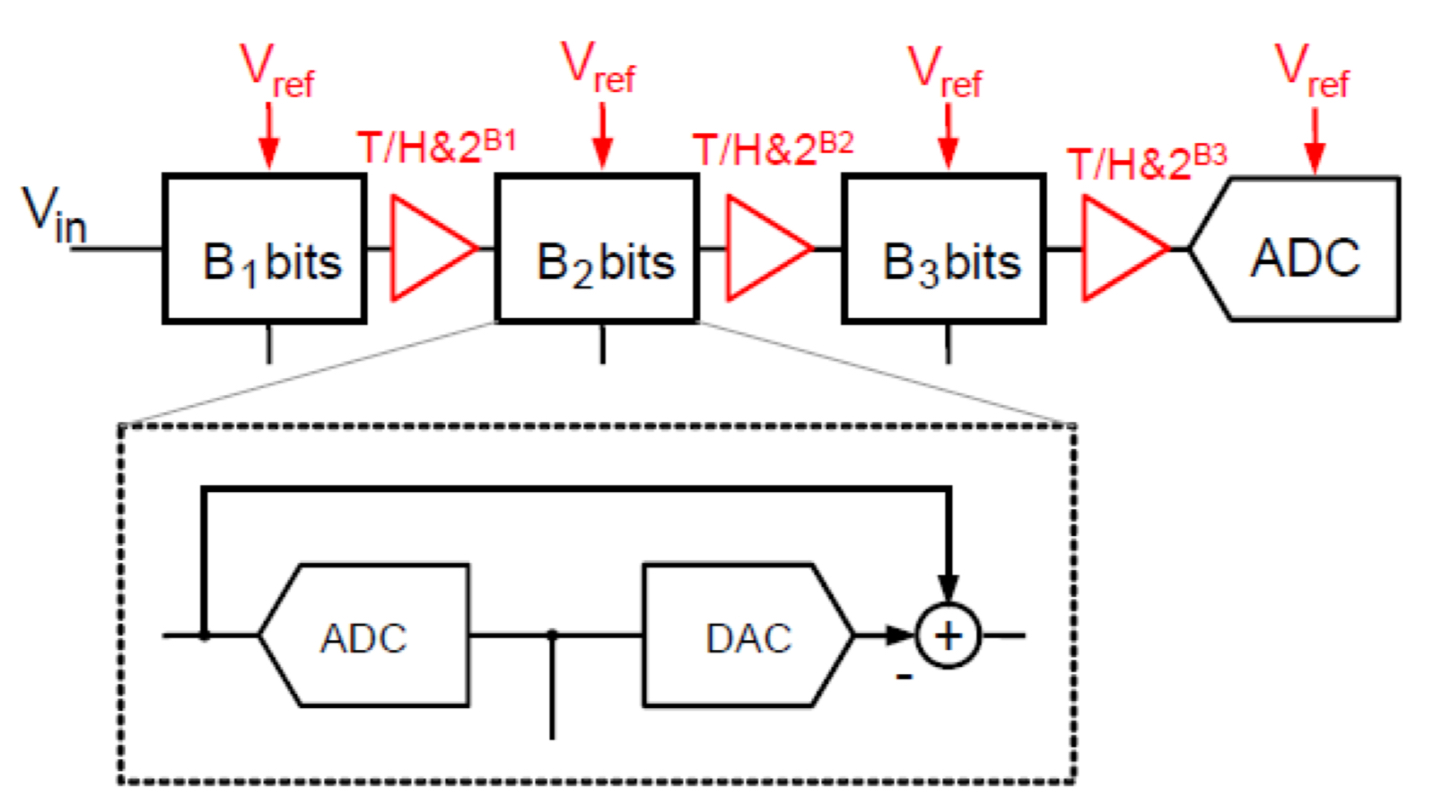
\includegraphics[width=0.5\textwidth]{figure/circuit1.jpg}
        		\caption{pipeline级联原理图} \label{fig:circuit1}
        	\end{figure}
        	
        总位数为
            \begin{equation}
                N=N_1+N_2+...-R
            \end{equation}
            
        N为总位数,其中R为冗余位。
        
        \textbf{\textit{在设计时需要注意以下几点:}}
        \begin{itemize}
			\item \textbf{时序设计基本原则:}$fs=1/Ts$,其中$Ts = min\{Ts_1,Ts_2,...\}$,由于采样率取决于最慢的周期,设计时尽量让每级周期近似相等,避免时序浪费。
			\item \textbf{余量传输:}如图\ref{fig:circuit2}所示,正常需要将数字量经过DAC转回模拟域,但考虑SAR采用电容开关阵列,可以加一位电容,利用SAR本身开关阵列实现DAC,得到余差。即纯SAR ADC的开关阵列正常需要N-2位电容,但若要利用电容开关阵列实现DAC功能,应当考虑N-1位电容,这就造成了前后级的结构不同,因为最后一级只需实现纯SAR ADC,无需再转换回模拟域。
				\begin{figure}[H]
					\centering
					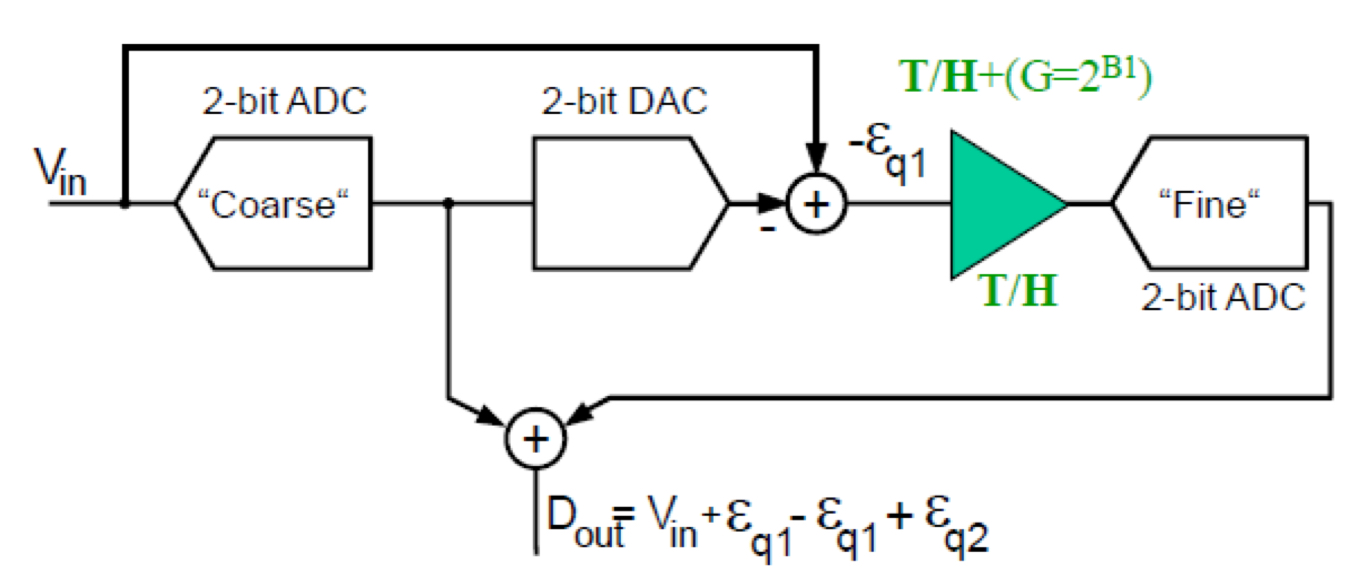
\includegraphics[width=0.7\textwidth]{figure/circuit2.jpg}
					\caption{余量放大传输原理图} \label{fig:circuit2}
				\end{figure}
			以2级流水线为例,若第一级M1位,第二级M2位,则实际第一级的ADC需要M1-1位电容,而第二即只需要M2-2位电容。
			\item \textbf{放大倍数:}
				\begin{equation}
					G=2^{M1-R-K}=2^{M1-R}\cdot\frac{Vref2}{Vref1}
				\end{equation}
			M1为前级ADC的位数。
			
			R为冗余位的位数——引入冗余的目的是为了采用冗余位校正算法来校正比较器失调和DAC建立误差,同时也能降低系统对比较器噪声的要求。
			
			k为两级间的缩减系数——例如第一级量化范围为$[0,Vref]$,第二级量化范围就可以表示为$[0,2^{-k} \cdot Vref]$,可以转化为两级参考电压之比。
			
			\item \textbf{冗余:}希望超出量化范围的信息也可以被后级SAR ADC量化。
			
			具体实现:余量放大器倍数减半并保持第二级SAR ADC量化范围不变,就可以实现1位冗余校正。
			
			模拟域和数字域对应:前级最高位和次级首位对齐,并减去失调。
			
			\item \textbf{运放误差:}运放非理想,实际情况需要考虑以下几方面的误差
				\begin{itemize}
					\item 有限增益误差
					\item 有限带宽误差
					\item 噪声和失调
				\end{itemize}
			
        \end{itemize}


    \subsection{Time-Interleaved ADC 建模原理}
		基本架构:如图\ref{fig:circuit3}所示,多路时间交织可以将等效采样率提高到但通道的m倍。
		\begin{figure}[H]
			\centering
			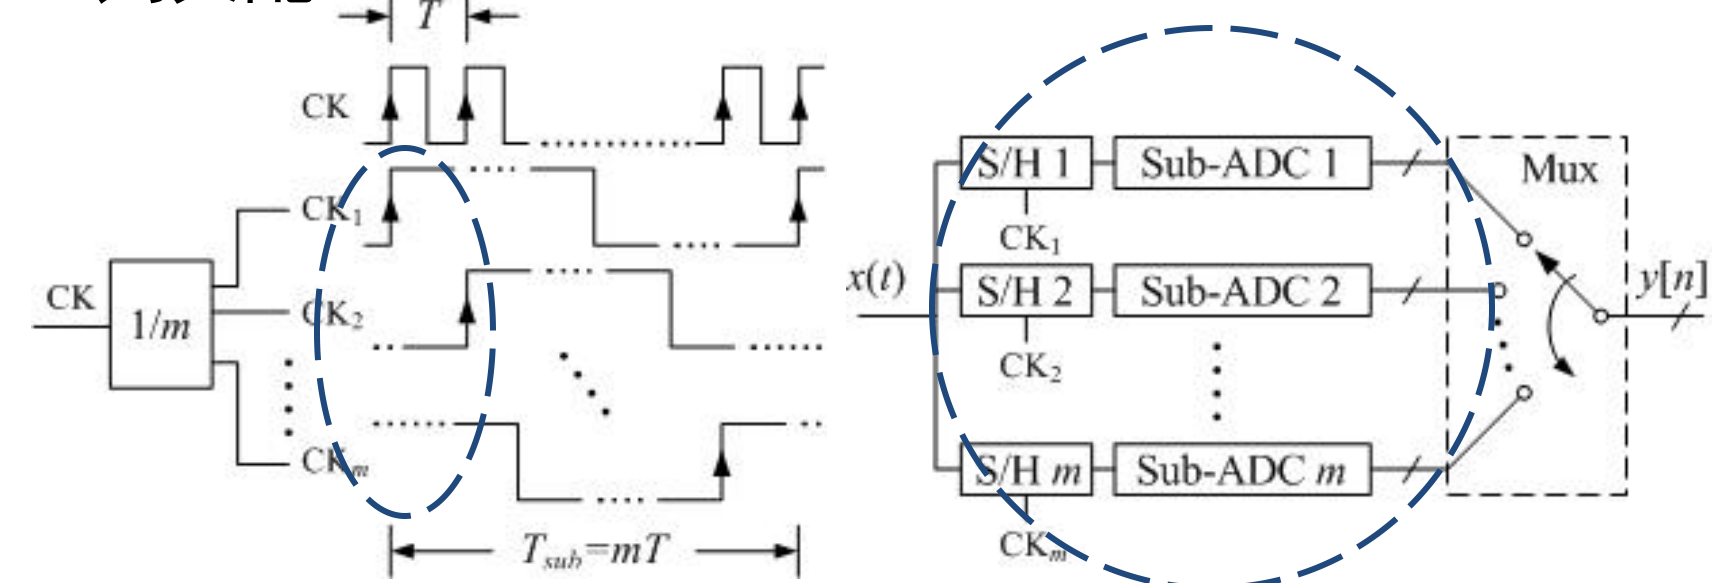
\includegraphics[width=1\textwidth]{figure/circuit3.png}
			\caption{时间交织原理及时序图} \label{fig:circuit3}
		\end{figure}
		\noindent
		\textbf{\textit{同样,注意建模设计要点:不同的通道间误差及其各自与频谱的对应关系}}
		在此,我们会首先回顾课上以两通道为例的失配,再将其推广到多通道,并研究不同通道间误差与频谱各自的对应关系。

		\subsubsection{失调失配}
		\textbf{以2通道为例,输入为 $x(t) = \cos(\omega t + \phi)$}
		\begin{itemize}
			\item \textbf{失调失配}:$x(t) = \cos(\omega t + \phi) + OS$
			\begin{itemize}
				\item 存在\textcolor{red}{失调}失配,$\Delta OS = OS_A - OS_B \neq 0$
				\item 量化结果:
				\[
				y[n] = \cos(\omega nT + \phi) + OS + \frac{\Delta OS}{2} \cos\left(\frac{\omega_s}{2} nT \right)
				\]
			\end{itemize}
		\end{itemize}
		\underline{\textbf{接下来,推广到多通道失调失配:}}
		\begin{equation}
			\begin{gathered}
				x_s(t)=x(t)+O(t)\\
				 \quad f_{I L}=k f_s / M \quad \text { where } k=0,1,2,3 \ldots, M-1 \\
				P_N=\frac{1}{M} \sum_{i=0}^{M-1}\left|O_i\right|^2
			\end{gathered}
		\end{equation}
		
		
		
		\subsubsection{增益失配}
		\textbf{增益失配}:$x(t) = G \cdot \cos(\omega t + \phi)$
		\begin{itemize}
			\item 存在\textcolor{red}{增益}失配,$\Delta G = G_A - G_B \neq 0$
			\item 量化结果:
			\[
			y[n] = G \cos(\omega nT + \phi) + \frac{\Delta G}{2} \cos\left[ \left(\omega - \frac{\omega_s}{2} \right) nT + \phi \right]
			\]
		\end{itemize}
		\underline{\textbf{接下来,推广到多通道增益失配:}}
		\begin{equation}
			\begin{gathered}
				x_s(t)=x(t) \times G(t) \\
				 f_{\text {Gain }} =k f_s / M \\
				f_{\text {IL }}=f_{\text {Gain }} \pm f_{\text {in }}= \pm f_{\text {in }}+\frac{k}{M} f_s \\
				 P_{\text {Total }}  =\frac{1}{2 M} \sum_{i=0}^{M-1}\left|G_i\right|^2
			\end{gathered}
		\end{equation}
		
		\subsubsection{时钟偏差}
		\textbf{采样时刻偏差}:$x(t) = \cos(\omega t + \phi + \Delta T)$
		\begin{itemize}
			\item 存在\textcolor{red}{采样时刻偏差},$\Delta T$
			\item 量化结果:
			\[
			y[n] = \cos\left(\frac{\omega \Delta T}{2}\right) \cos(\omega nT + \phi) + \sin\left(\frac{\omega \Delta T}{2}\right) \sin\left[\left(\omega - \frac{\omega_s}{2} \right) nT + \phi \right]
			\]
		\end{itemize}
		\underline{\textbf{接下来,推广到多通道采样时刻偏差:}}
		\begin{equation}
			\begin{array}{lr}
				x_s(t)=x(t-\delta t) & x_s(t)=\sin \left(2 \pi f_{i n} t\right) \cos \left(2 \pi f_{i n} \delta t\right)-\cos \left(2 \pi f_{i n} t\right) \sin \left(2 \pi f_{i n} \delta t\right) \\
				x(t)=\sin \left(2 \pi f_{i n} t\right) & x_s(t) \cong \sin \left(2 \pi f_{i n} t\right)-\left(2 \pi f_{i n} \delta t\right) \cos \left(2 \pi f_{i n} t\right) \\
				x_s(t)=\sin \left(2 \pi f_{i n} t-2 \pi f_{i n} \delta t \right) & f_{I L}= \pm f_{i n}+f_{\delta t}= \pm f_{i n}+\frac{k}{M} f_s \nonumber
			\end{array}
		\end{equation}
		
		\begin{equation}
			P_N=\frac{\left(2 \pi f_{i n}\right)^2}{2 M} \sum_{i=0}^{M-1}\left|\delta t_i\right|^2
		\end{equation}
		
		
		\subsubsection{带宽失配(但这个在本模型中未体现)}
		\textbf{带宽失配}:$x(t) = H(\omega) \cdot \cos(\omega t + \phi)$
		\begin{itemize}
			\item 存在\textcolor{red}{带宽}失配,$\Delta H(\omega) = H_A(\omega) - H_B(\omega) \neq 0$
			\item 量化结果:
			\[
			y[n] = H(\omega) \cos(\omega nT + \phi) + \frac{\Delta H(\omega)}{2} \cos\left[\left( \omega - \frac{\omega_s}{2} \right) nT + \phi \right]
			\]
		\end{itemize}
		\underline{\textbf{带宽失配未在本模型中加以考虑,只是在此做一个简单的说明}}
		
		\subsection{时间交织失配误差总结}
		\begin{flushleft}
					\begin{tabular}{|l|l|l|}
					\hline \textbf{Type of mismatch} & \textbf{Effect on input} & \textbf{Spur location} \\
					\hline Offset mismatch & Additive effect & $f_{\text {IL }}=\frac{k}{M} f_s$ \\
					\hline Gain mismatch & Amplitude modulation & $f_{\text {IL }}= \pm f_{\text {in }}+\frac{k}{M} f_s$ \\
					\hline Timing mismatch & Phase modulation & $f_{\text {IL }}= \pm f_{\text {in }}+\frac{k}{M} f_s$ \\
					\hline Bandwidth mismatch & Freq.-dependent amplitude and phase modulation & $f_{I L}= \pm f_{\text {in }}+\frac{k}{M} f_s$ \\
					\hline
				\end{tabular}
		\end{flushleft}
		
\section{MATLAB建模和仿真}
	\subsection{模型介绍}
	整体模型仿照硬件的结构进行搭建,主要包括以下几个部分:
	\begin{itemize}
		\item 顶层模型:
		实现整个时钟交织流水线SAR ADC的功能仿真。定义了ADC的整体参数和可能的噪声和失配,并生成测试用的正弦信号。
		ADC整体采用差分结构,因此需要生成两个共模相同,差模相反的正弦信号。
		模型首先对信号进行时钟交织的采样,采样时考虑了多通道间的时钟失配、增益失配、偏移量和kT/C噪声,将这些非理想因素叠加到输入信号中;
		接着调用多个流水线SAR ADC对多路采样数据进行并行化处理,考虑到了流水线ADC的各种噪声和失配,具体的因素会在每个模块中介绍;
		最后使用多路选择器将各个通道的量化结果整合得到更高采样率的量化结果。
		
		\item 流水线SAR ADC模型函数:
		实现流水线SAR ADC的功能仿真,以函数的形式被顶层模型调用。采用了两级流水的结构,并设置1位冗余位。
		考虑到噪声和失真的影响,采用了6位/8位的分布,使得最终的ENOB可以达到12位的设计要求。

		模型内部首先根据两级SAR ADC的位数求出两级所需要的电容值,并生成相应的电容阵列,电容阵列考虑到了寄生电容和电容大小失配。
		需要注意的是,第一级的余差在比较完成后还需要进一步缩小余差传递到第二级,
		而第二级的最后的余差在比较完成后不需要进一步处理,因此两级SAR ADC的实现方式有所不同,需要的电容数量也有所不同。
		具体而言,如果两级SAR ADC分别为N1位和N2位,则第一级SAR ADC的电容阵列需要N1+1个电容,而第二级SAR ADC的电容阵列只需要N2个电容。
		
		两级SAR ADC之间由一个余差放大器连接,使用反馈的形式控制余差的放大,将放大后的结果作为第二级SAR ADC的输入。

		最终的结果由两级SAR ADC的输出拼接得到。计算时将两级的冗余位重叠相加,并减去固定的偏移量得到最终的量化结果,输出到顶层模块进行多路整合。

		\item SAR ADC模型函数:
		模型的工作过程仿照SAR ADC的工作原理,使用循环模拟逐次逼近的过程,每次循环对输入的差分信号进行比较,并进行相应调整,考虑了比较器的失调和噪声。
		两级SAR ADC由于之前提到的原因,存在一些差别,需要分别设计。
		第一级ADC的电容阵列需要N1+1个电容,第二级ADC的电容阵列只需要N2个电容,并且第一级对输出余差电压的调整次数也比第二级多一次。其余部分两级完全相同。

		\item ResAmp模型函数:
		余差放大器将两个输入信号按照闭环增益进行放大,根据放大器的增益带宽积进行滤波后输出到第二级SAR ADC进行处理。
		输入的信号叠加了放大器的噪声和失调,闭环增益的计算也包含了有限增益带来的非线性因素。

		\item 静态参数测试函数
		实现对ADC静态参数的测试,包括DNL、INL指标的计算。由于输入是正弦信号,理想的histogram并不是均匀分布,而是呈“浴盆状”的分布曲线。
		函数通过使用大量数据模拟得到理想的概率分布,再用实际得到的概率分布与理想分布相减得到DNL,对DNL积分得到INL。

		\item 动态参数测试函数
		实现对ADC动态参数的测试,包括SNR、SFDR、THD、SNDR和ENOB指标的计算。函数通过对输入的正弦信号进行FFT变换,得到频谱图,
		去除DC分量后找到能量最大的频率作为主频,将主频乘以整数倍的频率作为谐波,取2-5次谐波进行计算。
		计算主频和谐波的功率比得到THD,将2次谐波功率与主频功率的比得到SFDR。
		去除DC、主频和谐波后,计算剩余部分的功率就是噪声功率,主频功率与噪声功率之比就是SNR。
		主频功率比上噪声功率与谐波功率之和就是SNDR,由此可以计算出ENOB。由于各种噪声和失真,ENOB小于最初设计的13位,但仍然满足12位的要求。

	\end{itemize}
	\subsection{仿真参数}
	在本节中,我们将对上述模型进行仿真,主要关注以下几个方面的参数设置:
	\subsubsection{模型参数}
	\begin{itemize}
		\item \textbf{采样频率}:$f_s = 2 \text{GHz}$
		\item \textbf{参考电压幅度}:$V_{ref} = 1.8V$
		\item \textbf{共模电压}:$V_{cm} = 0.9V$
		\item \textbf{ADC位数}:$N = 13$,这是ADC的理想位数。
		\item \textbf{通道数}:$M = 4$,这是时间交织ADC的通道数。
		\item \textbf{非理想指标}:包括时钟jitter、增益失配、偏移失调等,这些参数将在仿真中逐步调整。
	\end{itemize}

	\subsubsection{采样与输入信号参数}
	\begin{itemize}
		\item \textbf{采样点数}:$num = 2^{15}$,这是整个ADC的采样点数。由于理想位数为13位,为了完整测量,采样了$2^{15}$,无法采样更多是因为matlab内存不允许。
		\item \textbf{输入信号频率}:$f_{in} = \frac{1517}{num} * fs$,未超过奈奎斯特频率,且与采样频率$f_s$互质,以免DNL测量出现-1。同时采样$num$点正好是整周期,可以不进行加窗。
		\item \textbf{输入信号幅度}:$V_{in} = 1.0$,这是输入正弦信号的幅度。
	\end{itemize}

	\subsection{仿真结果}
	在本节中,我们将展示基于上述模型和参数在不同情况下的仿真结果,包括静态参数和动态参数的测试结果。
	\subsubsection{理想情况}
	在没有任何失配、失调等情况下,我们可以得到理想的ADC性能。可以看到最差DNL为0.59LSB,最差INL为0.78LSB,SNR为80.01dB,SNDR为80.01dB,SFDR为82dB,THD为105.12dB,ENOB为13bit。
		\begin{figure}[H]
			\centering
			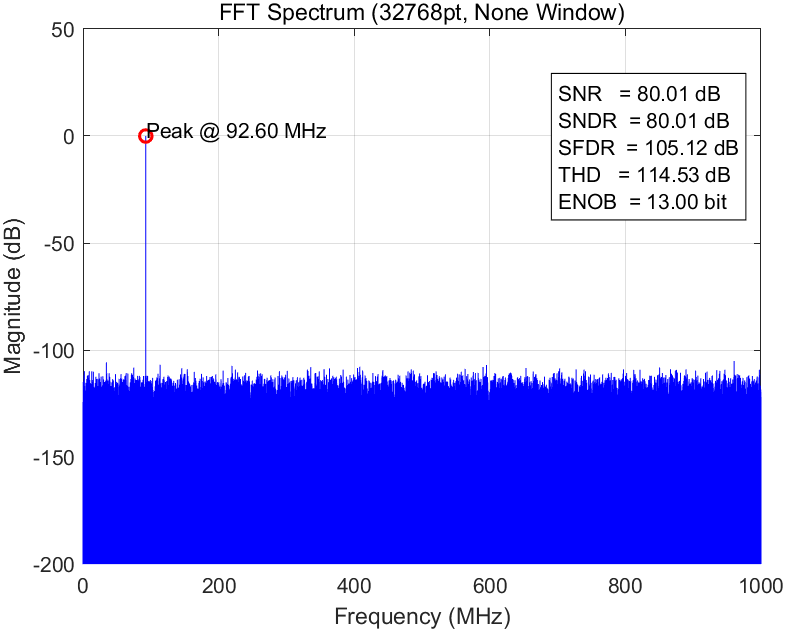
\includegraphics[width=0.7\textwidth]{pic/ideal/DFT.png}
			\caption{理想情况下的动态特性} 
		\end{figure}

		\begin{figure}[H]
			\centering
			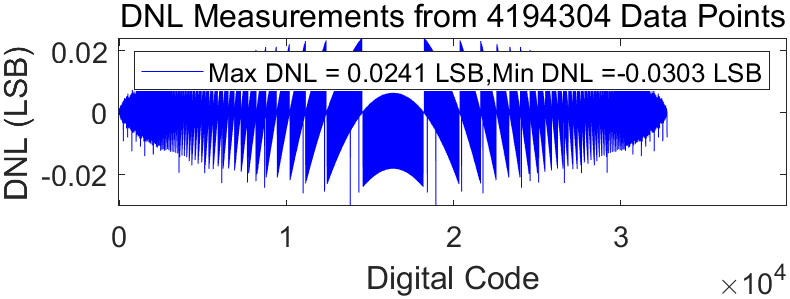
\includegraphics[width=0.7\textwidth]{pic/ideal/DNL.png}
			\caption{理想情况下的DNL} 
		\end{figure}

		\begin{figure}[H]
			\centering
			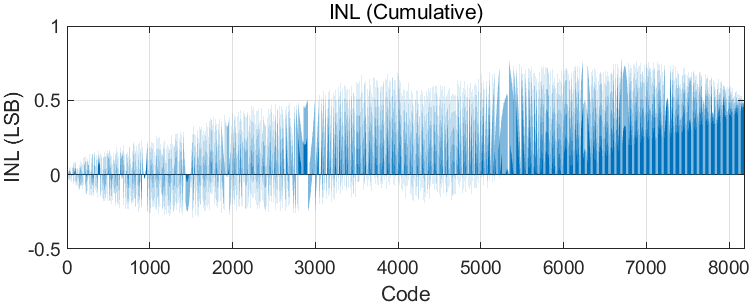
\includegraphics[width=0.7\textwidth]{pic/ideal/INL.png}
			\caption{理想情况下的INL} 
		\end{figure}

		\begin{figure}[H]
			\centering
			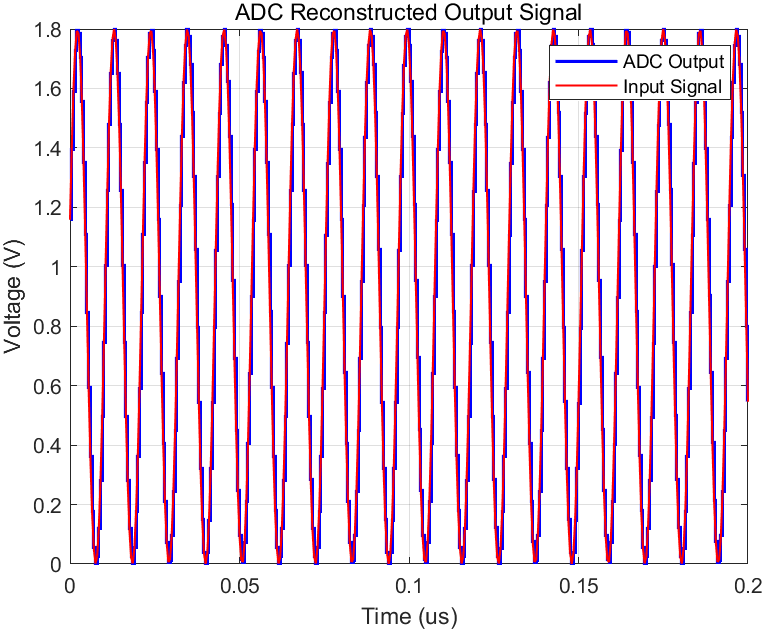
\includegraphics[width=0.7\textwidth]{pic/ideal/inout.png}
			\caption{理想情况下的输入输出对比} 
		\end{figure}

	\subsubsection{TI mismatch}
	\begin{itemize}
		\item \textbf{失调失配} 设置四个通道各自有$Mis_{OS} = 0.5 * LSB * randn()$;此时ADC性能。可以看到最差DNL为1LSB,最差INL为1.2LSB,SNR为78.52dB,SNDR为78.52dB,SFDR为83.9dB,THD为126.97dB,ENOB为12.75bit。

		\begin{figure}[H]
			\centering
			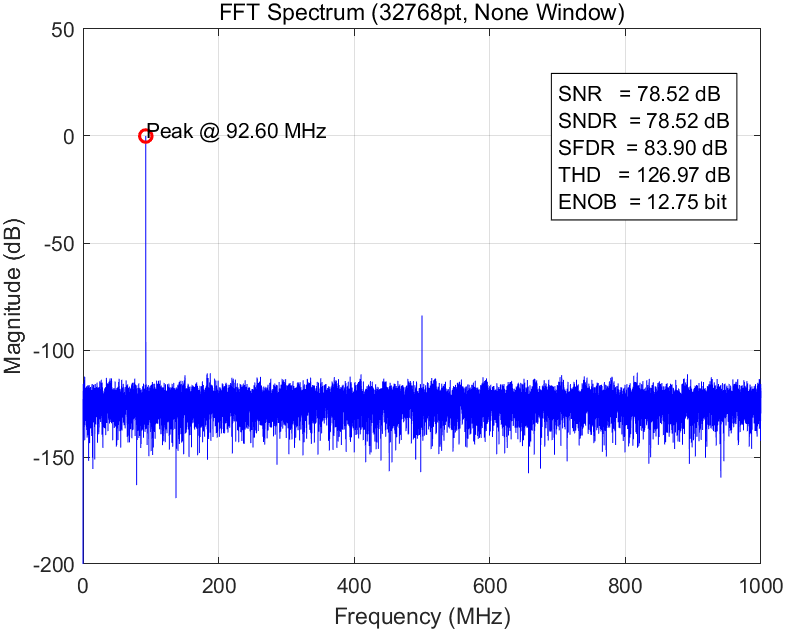
\includegraphics[width=0.7\textwidth]{pic/TIOS/DFT.png}
			\caption{通道内存在失调失配下的动态特性} 
		\end{figure}

		\begin{figure}[H]
			\centering
			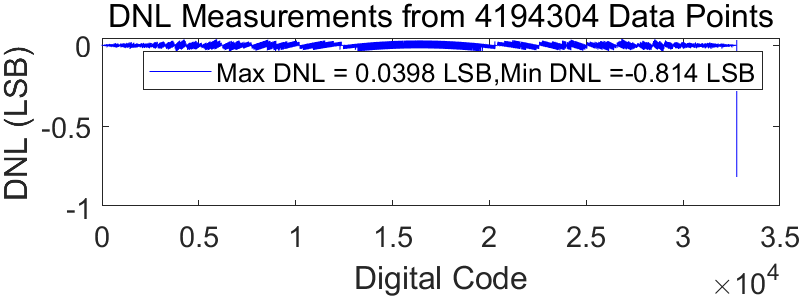
\includegraphics[width=0.7\textwidth]{pic/TIOS/DNL.png}
			\caption{通道内存在失调失配下的DNL} 
		\end{figure}

		\begin{figure}[H]
			\centering
			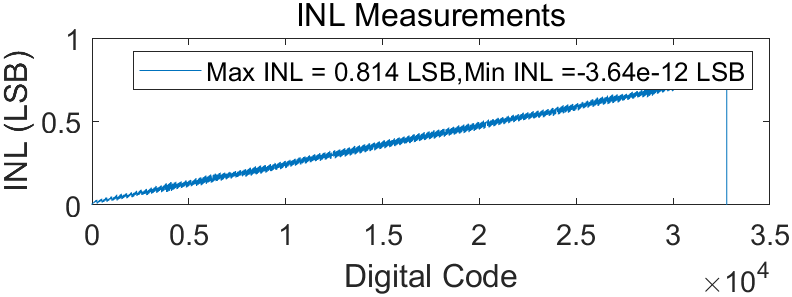
\includegraphics[width=0.7\textwidth]{pic/TIOS/INL.png}
			\caption{通道内存在失调失配下的INL} 
		\end{figure}

		\item \textbf{增益失配} 设置四个通道各自有$Mis_{Gain} = 1 + 0.2 * randn()$;
		\begin{figure}[H]
			\centering
			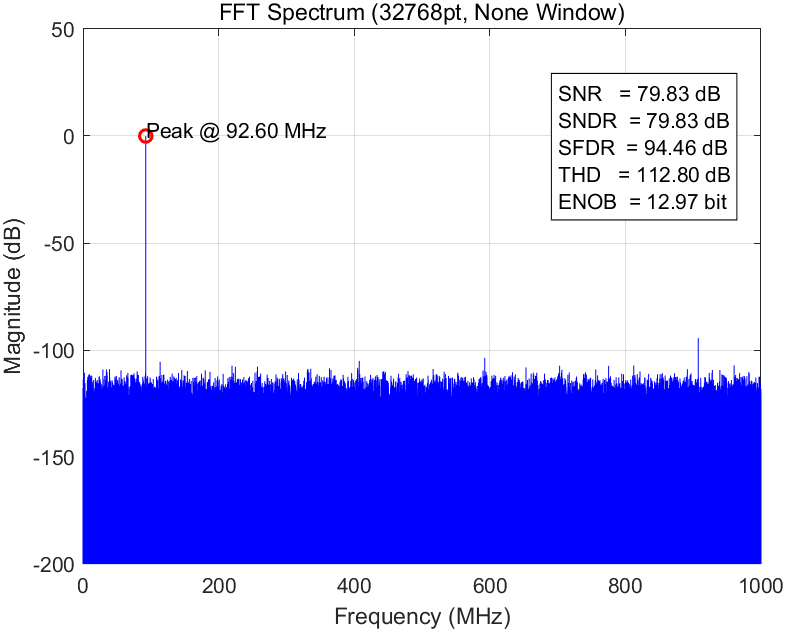
\includegraphics[width=0.7\textwidth]{pic/TIG/DFT.png}
			\caption{通道内存在增益失配下的动态特性} 
		\end{figure}

		\begin{figure}[H]
			\centering
			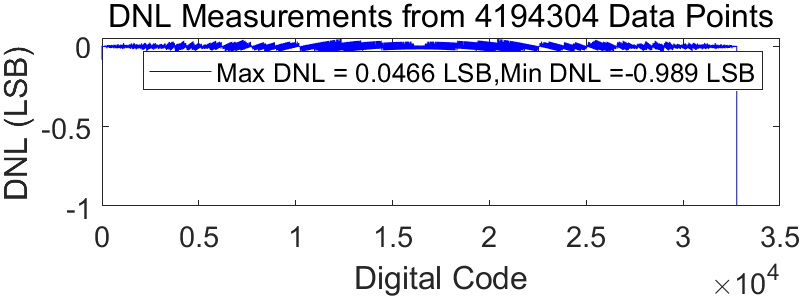
\includegraphics[width=0.7\textwidth]{pic/TIG/DNL.png}
			\caption{通道内存在增益失配下的DNL} 
		\end{figure}

		\begin{figure}[H]
			\centering
			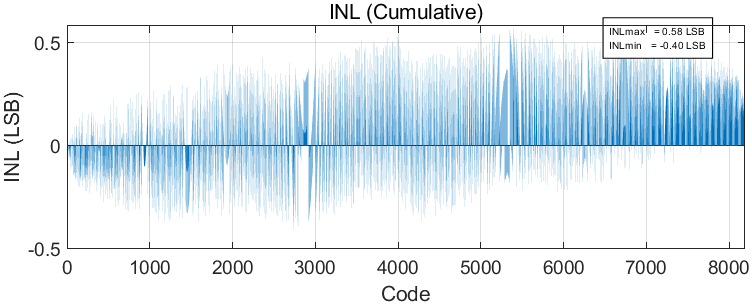
\includegraphics[width=0.7\textwidth]{pic/TIG/INL.png}
			\caption{通道内存在增益失配下的INL} 
		\end{figure}

		\item \textbf{时钟偏差} 设置四个通道各自有$Mis_{Clk} = 0.005 * 1/fs * randn()$;
		\begin{figure}[H]
			\centering
			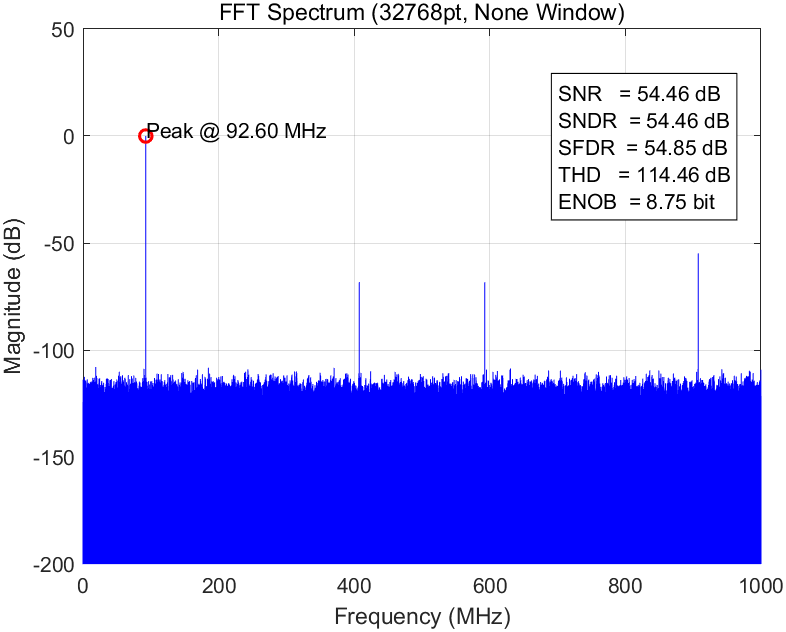
\includegraphics[width=0.7\textwidth]{pic/TIC/DFT.png}
			\caption{通道间存在时钟偏差下的动态特性} 
		\end{figure}

		\begin{figure}[H]
			\centering
			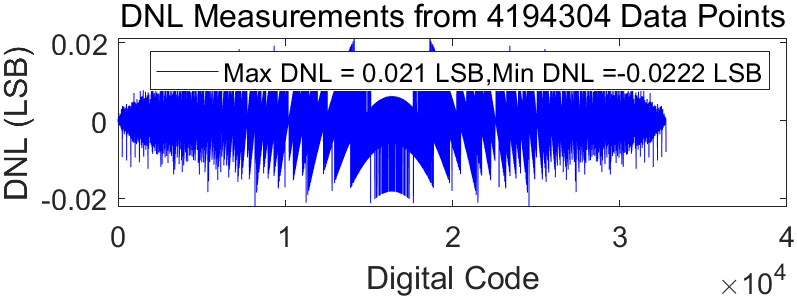
\includegraphics[width=0.7\textwidth]{pic/TIC/DNL.png}
			\caption{通道间存在时钟偏差下的DNL} 
		\end{figure}

		\begin{figure}[H]
			\centering
			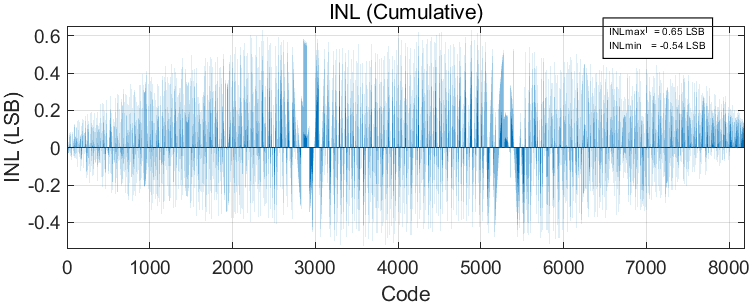
\includegraphics[width=0.7\textwidth]{pic/TIC/INL.png}
			\caption{通道间存在时钟偏差下的INL} 
		\end{figure}
	\end{itemize}

	\subsubsection{pipelined-SAR ADC级间运放误差}
	\begin{itemize}
		\item \textbf{有限增益误差(级间增益误差)} 级间增益误差可以通过改变级间增益放大器的开环增益来实现,当开环增益非正无穷时,级间增益为理想的$2^6=64$。将开环增益改为60dB,实际级间增益为$\frac{1000}{1+1000*\frac{1}{2^6}}=60.15$。
		\begin{figure}[H]
			\centering
			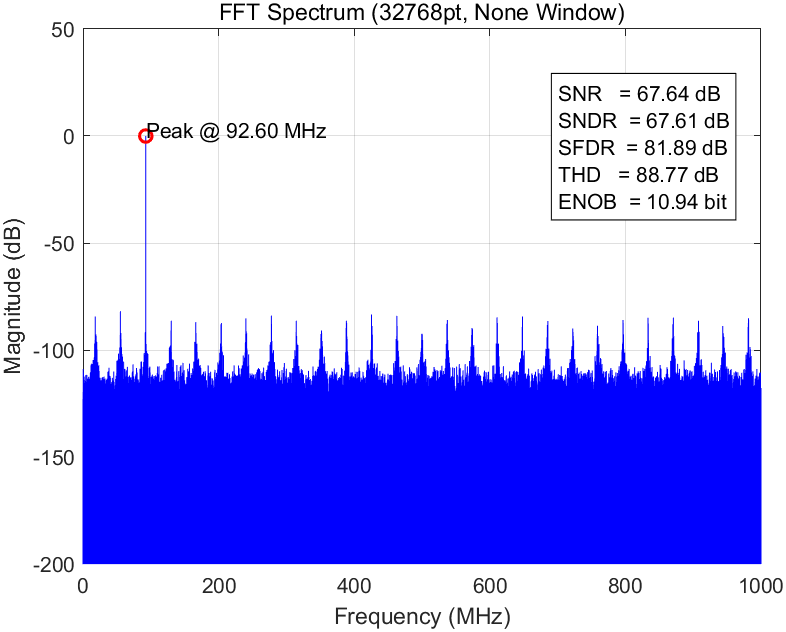
\includegraphics[width=0.7\textwidth]{pic/Av/DFT.png}
			\caption{有限增益误差下的动态特性} 
		\end{figure}

		\begin{figure}[H]
			\centering
			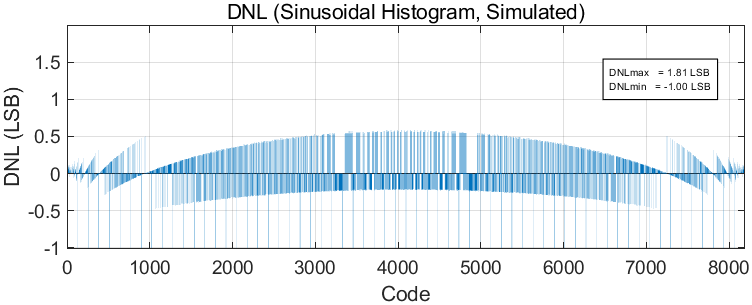
\includegraphics[width=0.7\textwidth]{pic/Av/DNL.png}
			\caption{有限增益误差下的DNL} 
		\end{figure}

		\begin{figure}[H]
			\centering
			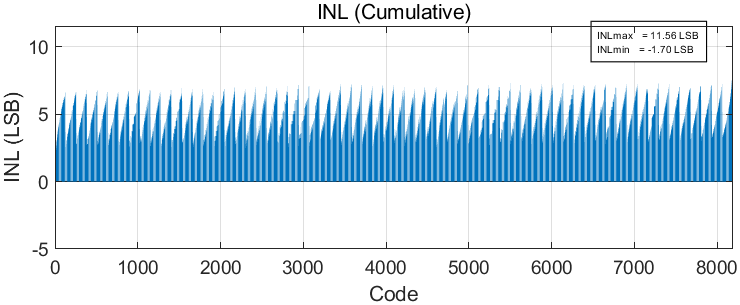
\includegraphics[width=0.7\textwidth]{pic/Av/INL.png}
			\caption{有限增益误差下的INL} 
		\end{figure}

		\item \textbf{有限带宽误差} 理想情况时级间增益放大器的带宽为$10GHz$,现将带宽设置为为$2GHz$。
		\begin{figure}[H]
			\centering
			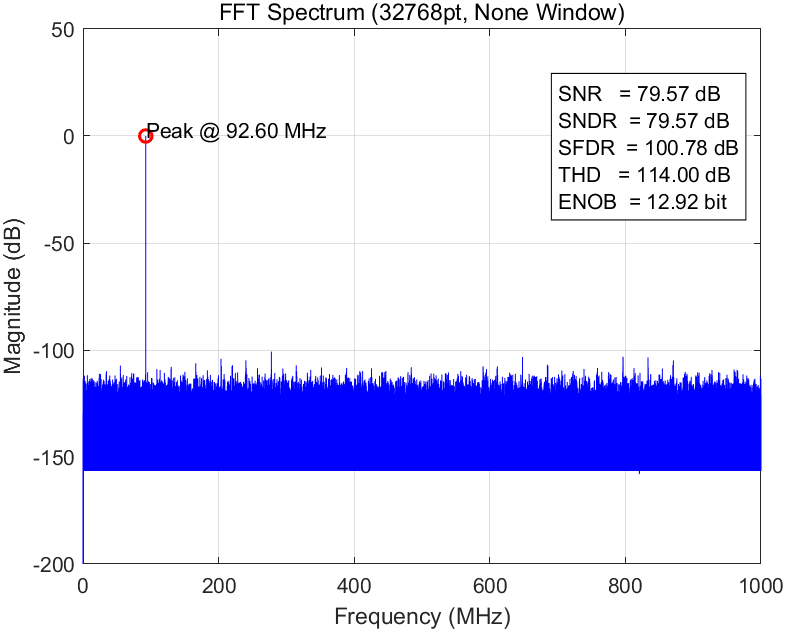
\includegraphics[width=0.7\textwidth]{pic/GBW/DFT.png}
			\caption{有限带宽误差下的动态特性} 
		\end{figure}

		\begin{figure}[H]
			\centering
			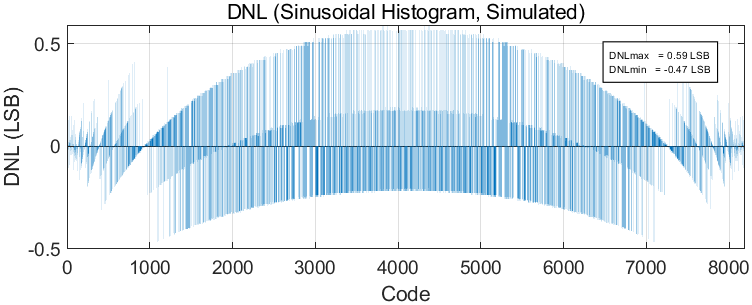
\includegraphics[width=0.7\textwidth]{pic/GBW/DNL.png}
			\caption{有限带宽误差下的DNL} 
		\end{figure}

		\begin{figure}[H]
			\centering
			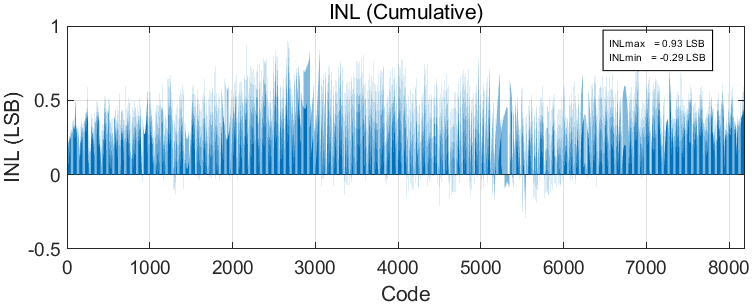
\includegraphics[width=0.7\textwidth]{pic/GBW/INL.png}
			\caption{有限带宽误差下的INL} 
		\end{figure}

		\item \textbf{运放噪声与失调} 将失调调为0.001V,噪声设置为$0.001V*randn()$。???理论来说如此小的失调应该会被冗余遮盖
		\begin{figure}[H]
			\centering
			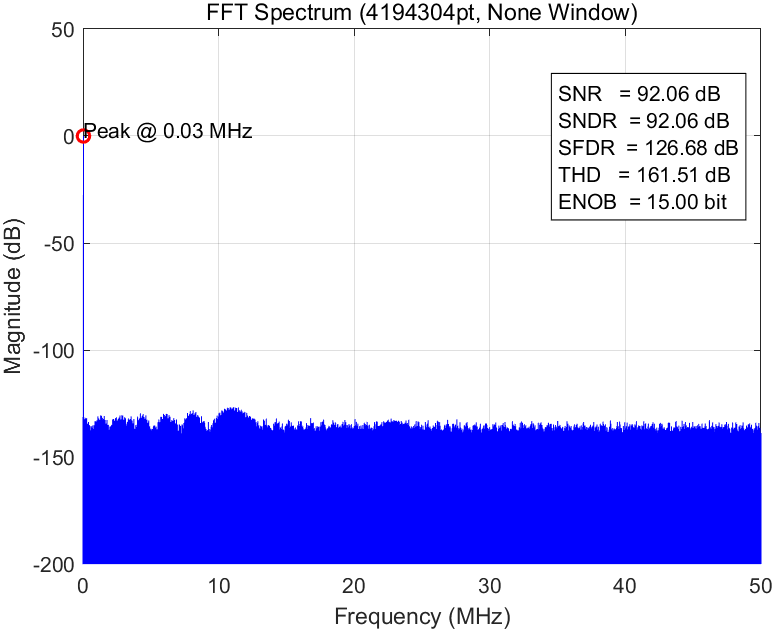
\includegraphics[width=0.7\textwidth]{pic/Avno/DFT.png}
			\caption{存在运放噪声与失调时的动态特性} 
		\end{figure}

		\begin{figure}[H]
			\centering
			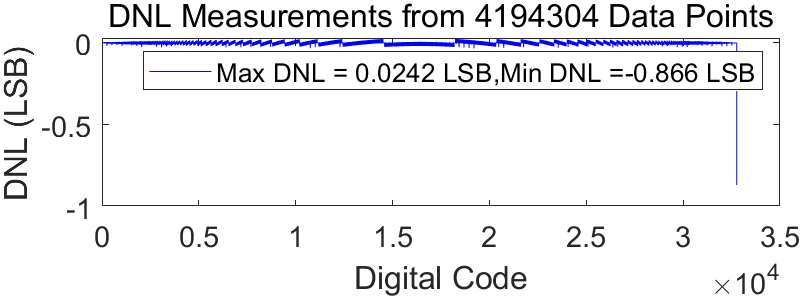
\includegraphics[width=0.7\textwidth]{pic/Avno/DNL.png}
			\caption{存在运放噪声与失调时的DNL} 
		\end{figure}

		\begin{figure}[H]
			\centering
			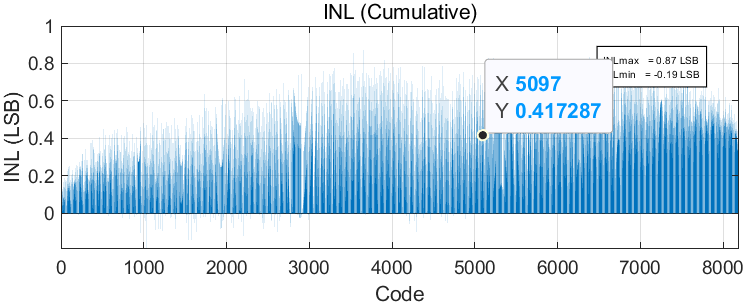
\includegraphics[width=0.7\textwidth]{pic/Avno/INL.png}
			\caption{存在运放噪声与失调时的INL} 
		\end{figure}

	\end{itemize}

\subsubsection{SAR ADC非理想}
	\begin{itemize}
		\item \textbf{比较器失调与噪声} 将失调调为0.005V,噪声设置为$0.005V*randn()$。
		\begin{figure}[H]
			\centering
			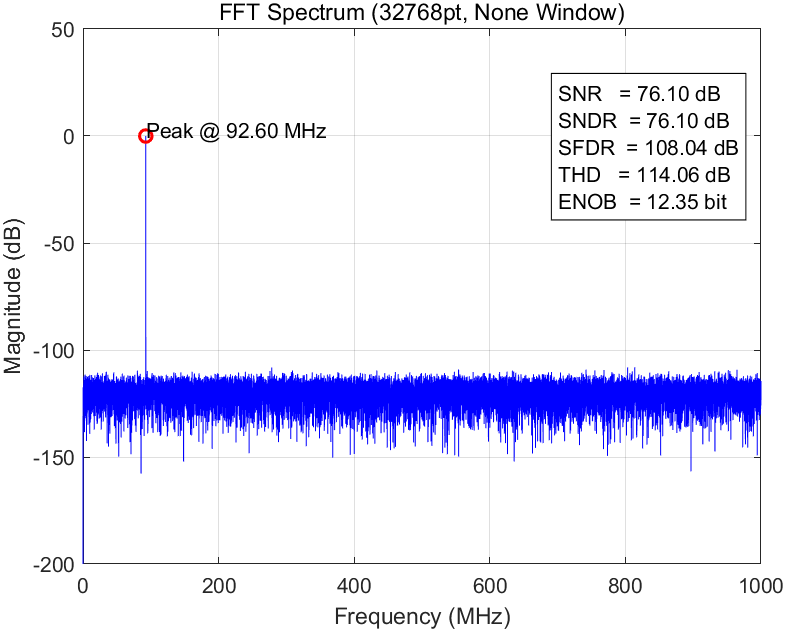
\includegraphics[width=0.7\textwidth]{pic/Comno/DFT.png}
			\caption{存在比较器失调与噪声的动态特性} 
		\end{figure}

		\begin{figure}[H]
			\centering
			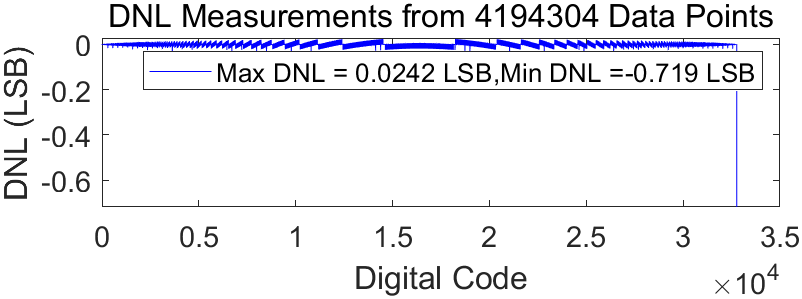
\includegraphics[width=0.7\textwidth]{pic/Comno/DNL.png}
			\caption{存在比较器失调与噪声的DNL} 
		\end{figure}

		\begin{figure}[H]
			\centering
			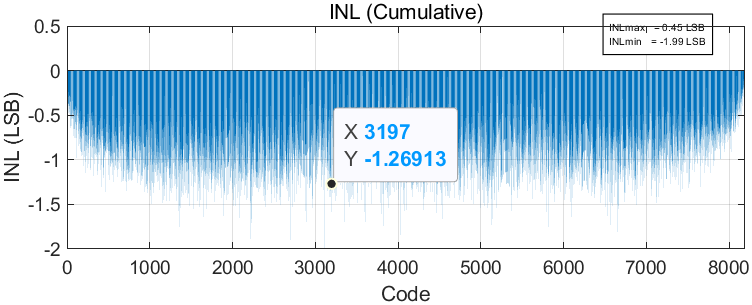
\includegraphics[width=0.7\textwidth]{pic/Comno/INL.png}
			\caption{存在比较器失调与噪声的INL} 
		\end{figure}

		\item \textbf{寄生电容} 先将第一级的寄生电容调为$Cp_{p1}  = 5fF $、$ Cp_{n1} = 5fF;$ 
		\begin{figure}[H]
			\centering
			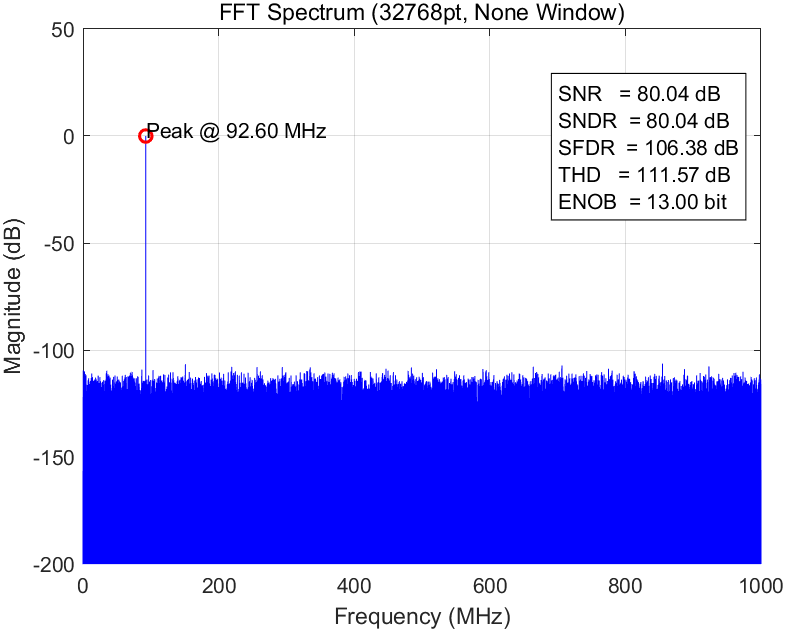
\includegraphics[width=0.7\textwidth]{pic/Co/DFT1.png}
			\caption{第一级寄生电容的动态特性} 
		\end{figure}

		\begin{figure}[H]
			\centering
			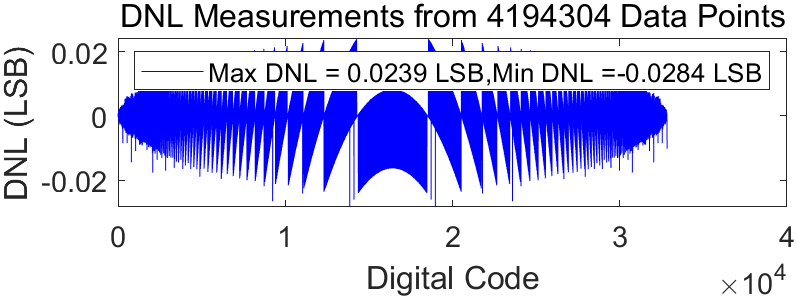
\includegraphics[width=0.7\textwidth]{pic/Co/DNL1.png}
			\caption{第一级寄生电容的DNL} 
		\end{figure}

		\begin{figure}[H]
			\centering
			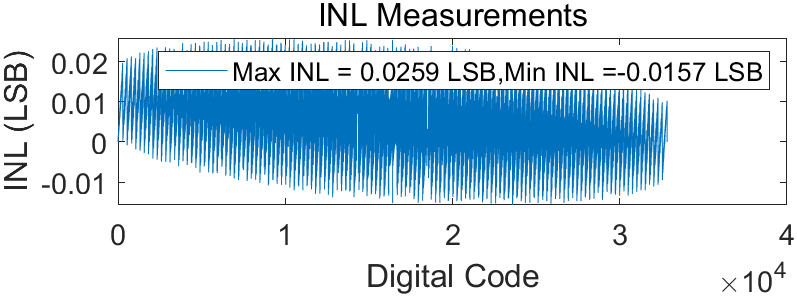
\includegraphics[width=0.7\textwidth]{pic/Co/INL1.png}
			\caption{第一级寄生电容的INL} 
		\end{figure}

		再将第二级的寄生电容调为$Cp_{p2}  = 5fF $、$ Cp_{n2} = 5fF;$
		\begin{figure}[H]
			\centering
			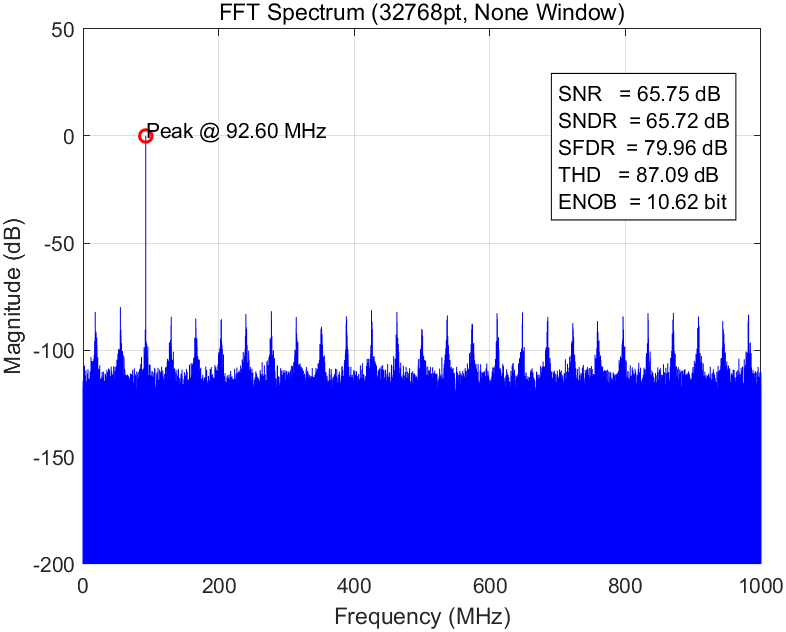
\includegraphics[width=0.7\textwidth]{pic/Co/DFT2.png}
			\caption{第二级寄生电容的动态特性}
		\end{figure}

		\begin{figure}[H]
			\centering
			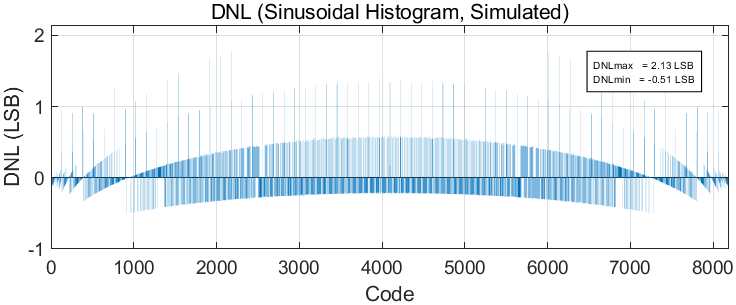
\includegraphics[width=0.7\textwidth]{pic/Co/DNL2.png}
			\caption{第二级寄生电容的DNL}
		\end{figure}

		\begin{figure}[H]
			\centering
			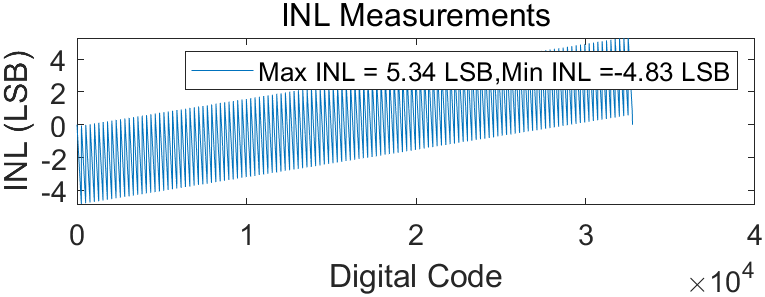
\includegraphics[width=0.7\textwidth]{pic/Co/INL2.png}
			\caption{第二级寄生电容的INL}
		\end{figure}

		\item \textbf{电阻热噪声} 测量T=300k时的电阻热噪声
		\begin{figure}[H]
			\centering
			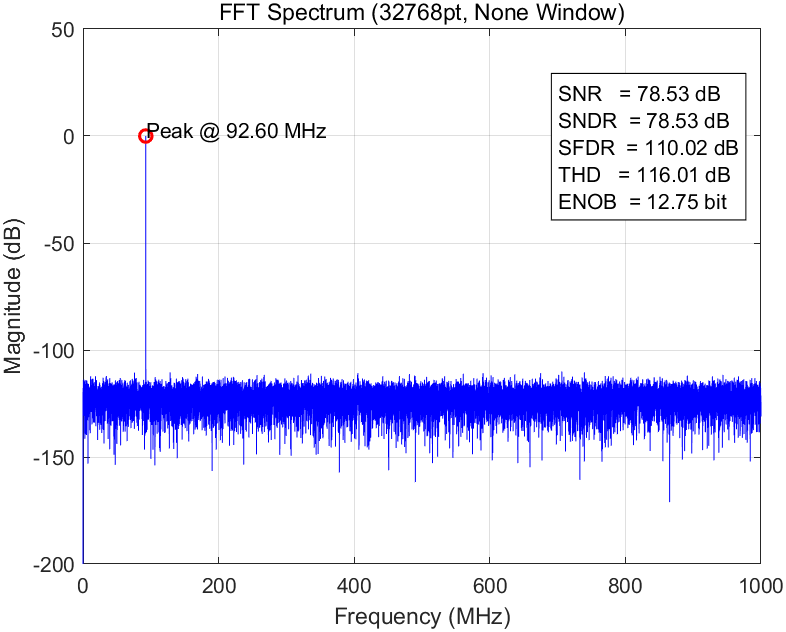
\includegraphics[width=0.7\textwidth]{pic/KT/DFT.png}
			\caption{电阻热噪声的动态特性} 
		\end{figure}

		\begin{figure}[H]
			\centering
			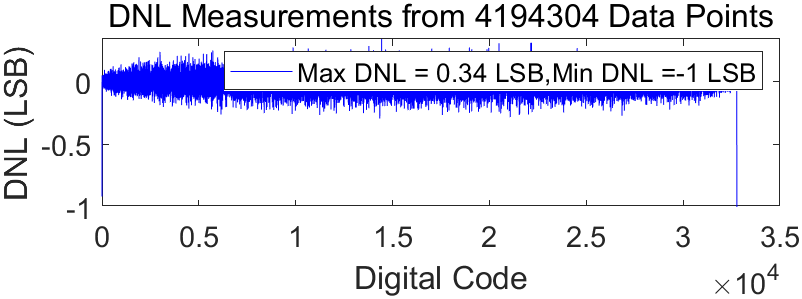
\includegraphics[width=0.7\textwidth]{pic/KT/DNL.png}
			\caption{电阻热噪声的DNL} 
		\end{figure}

		\begin{figure}[H]
			\centering
			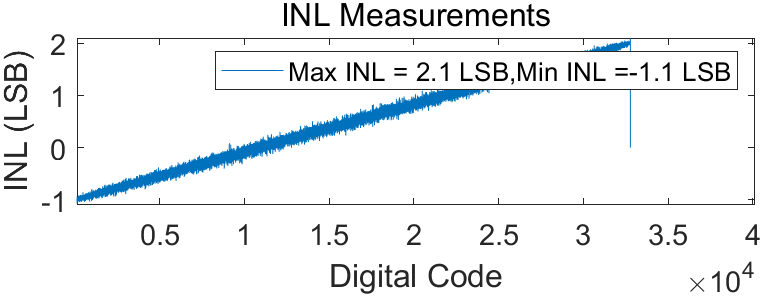
\includegraphics[width=0.7\textwidth]{pic/KT/INL.png}
			\caption{电阻热噪声的INL} 
		\end{figure}
	\end{itemize}


\subsubsection{所有非理想叠加}
$Mis_{OS} = 0.5 * LSB * randn()$;

$Mis_{Gain} = 1 + 0.2 * randn()$;

$Mis_{Clk} = 0.005 * 1/fs * randn()$;

实际级间增益为60.15;

带宽设置为为$2GHz$;

运放失调调为0.001V,噪声设置为$0.001V*randn()$;

比较器失调调为0.005V,噪声设置为$0.005V*randn()$;

第一级的寄生电容调为$Cp_{p1}  = 5fF $、$ Cp_{n1} = 5fF;$ 

第二级的寄生电容调为$Cp_{p2}  = 5fF $、$ Cp_{n2} = 5fF;$ 

T=300k时的电阻热噪声。
		\begin{figure}[H]
			\centering
			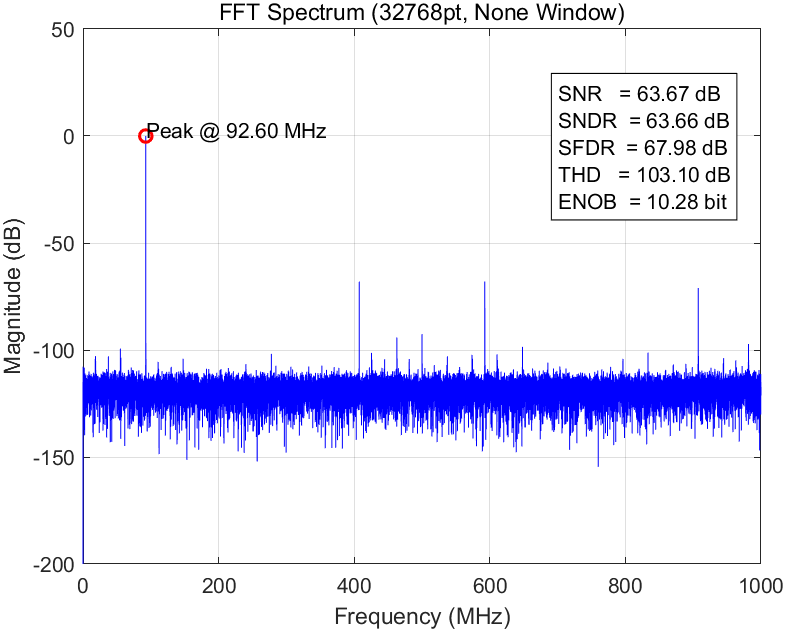
\includegraphics[width=0.7\textwidth]{pic/noideal/DFT.png}
			\caption{全都非理想时的动态特性} 
		\end{figure}

		\begin{figure}[H]
			\centering
			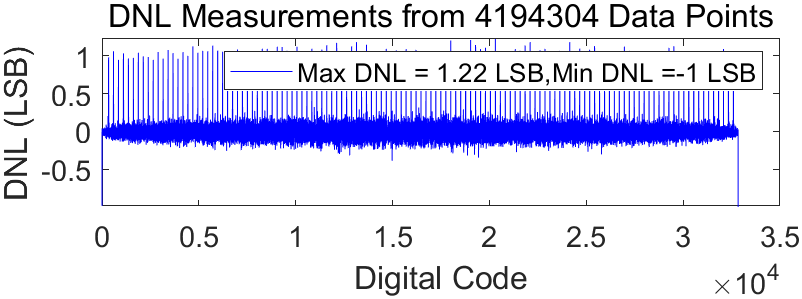
\includegraphics[width=0.7\textwidth]{pic/noideal/DNL.png}
			\caption{全都非理想时的DNL} 
		\end{figure}

		\begin{figure}[H]
			\centering
			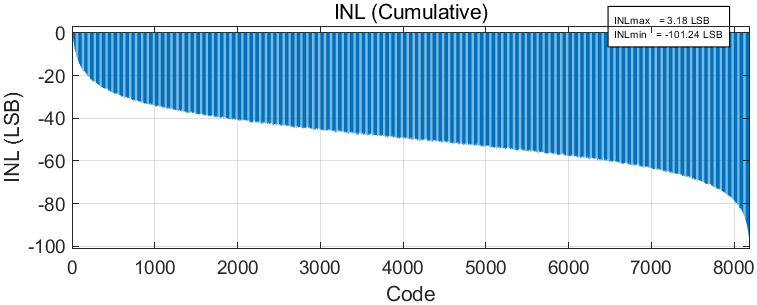
\includegraphics[width=0.7\textwidth]{pic/noideal/INL.png}
			\caption{全都非理想时的INL} 
		\end{figure}


%============= 参考文献 =====================
% \addcontentsline{toc}{section}{参考文献}
% \bibliography{bibfile}
\clearpage
%=============  致谢  ======================
% \include{body/acknowledge}
%\include{body/appendices}

\end{document}
%%%%%%%%%% 结束 %%%%%%%%%%